\section{Mod\'eliser la coh\'erence de cache}
\label{fr:sec:model}

Cette section offre un aperçu du modèle UPPAAL\footnote{Disponible sur
\url{https://github.com/nsensfel/phylog-cache-coherence}} pour l'analyse des
effets de la cohérence de cache dans les processeurs multi-cœurs. Sont but est
de créer un modèle formel afin de pouvoir faire des analyses automatiques
(décrites dans la Section~\ref{fr:sec:analyze}) tout en assurant que:
\begin{itemize}
  \setlength{\itemsep}{0pt}%
   \setlength{\parskip}{0pt}%
\item Le modèle est aussi générique que possible dans la façon dont il modélise
la cohérence de cache afin de permettre de facilement passer d'un protocole à
un autre.
\item Les protocoles sont modélisés en détails, prenant en compte tous les états
transitoires et sont définis pour des bus \textit{split-transaction}.
\end{itemize}

L'approche choisie est similaire à celles des papiers présentés dans
la Section~\ref{fr:sec:rel_formal}: utiliser un réseau d'automates de
tailles modérées, chacun représentant un composant, afin que le système
résultant soit facile à comprendre et modulaire.

\subsection{Stratégie de modélisation}
\label{fr:sec:modeling:strategy}
% Pour créer un modèle de l'architecture, la solution choisie a été de la baser
% sur les principes expliqués dans la Section~\ref{fr:sec:cache_coherence}.
Le modèle de l'architecture est limité aux éléments directement liés
à la cohérence de cache. On suppose qu'un applicant ayant besoin de
composants plus précis ou de composants additionnels peut soit les
prendre depuis une autre solution, soit intégrer les composants de
cohérence de cache présents ici dans cette autre solution.

Chaque composant a son propre automate. Les états et transitions de chaque automate représentent en premier lieu les communications (via des synchronisations) entre les différents composants. Le fonctionnement interne de chaque composant, comme les états de cohérence, est décrit via des variables d'états qui sont mises à jour dans des fonctions, qui utilisent une
syntaxe proche du C d'UPPAAL. Cela produite des automates plus
petits et plus lisibles, car les transitions sont moins nombreuses et
leur actions sont faites par l'appel à des fonctions au nom
significatif.

\begin{figure}[hbt!]
\begin{center}
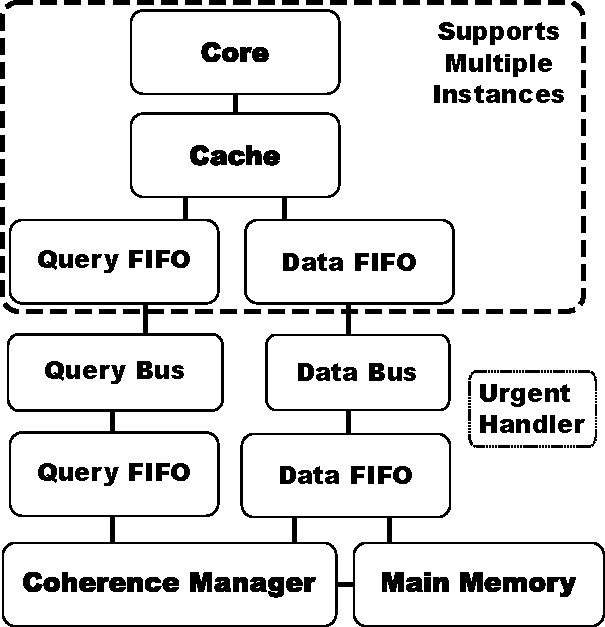
\includegraphics[width=0.5\textwidth]{\chapterdirectory/figure/model_overview.pdf}
\end{center}
\caption{Vue d'ensemble des automates du modèle}
\label{fr:fig:UPPAAL:automata_overview}
\end{figure}

La Figure~\ref{fr:fig:UPPAAL:automata_overview} montre tous les automates
définis dans le modèle. On y retrouve les composants d'une architecture multi-coœurs, plus quelques artefacts de modélisation. En effet,
l'interconnect \textit \textit{split-transaction} a été divisé en deux
composantes: un bus de demande et un bus de réponse. De plus, un automate de
file de messages FIFO pour les réponses a été ajouté et est partagé par le
gestionnaire de cohérence et le contrôleur mémoire. Pour finir, un automate
\textit{Urgent Handler} est présent, qui ne correspond à aucun composant
physique mais permet de faire des synchronisations \texttt{urgent}.

% Pour faciliter les communications, un identifiant unique est assigné a certains
% des composants (les caches, les cœurs, le gestionnaire de cohérence, le
% contrôleur mémoire et le bus de demandes). Cet identifiant est utilisé pour la
% sélection du sous canal approprié dans certaines synchronisations, ainsi que
% pour l'identification de l'envoyeur et du receveur des messages. De plus, cela
% permet de préciser dans la déclaration du système à quel automates un automate
% devrait se connecter, en passant l'identifiant des automates cibles comme
% paramètre (par exemple un cache et ses files de messages).

Les transferts de données entre automates sont faits par synchronisation:
l'émetteur stocke la valeur dans une variable globale, qui est lue par le ou
les receveurs. Cette variable globale est définie de manière à clairement
identifier l'émetteur et, s'il y a lieu, le receveur. L'élément mémoire concerné
par l'échange est aussi indiqué dans cette variable globale, ainsi que le type
de message (par exemple \texttt{GetM}). La validité de cette variable globale
n'est assurée que le temps de la transition, puisque la prochaine transition
peut en changer le contenu. En conséquent, les automates la recevant vont
garder une copie du message dans une variable locale.

% \begin{figure}[hbt!]
% \begin{center}
% \begin{tikzpicture}[
  font=\sffamily,
  every matrix/.style={ampersand replacement=\&,column sep=2cm,row sep=2cm},
  source/.style={draw,thick,rounded corners,fill=yellow!20,inner sep=.3cm},
  process/.style={draw,thick,circle,fill=blue!20},
  sink/.style={source,fill=green!20},
  datastore/.style={draw,very thick,shape=datastore,inner sep=.3cm},
  dots/.style={gray,scale=2},
  to/.style={->,>=stealth',shorten >=1pt,semithick,font=\sffamily\footnotesize},
  every node/.style={align=center}]

  % Position the nodes using a matrix layout
  \matrix{
    \node[source] (core0) {Core 0};
      \& \node[source] (cache0) {Cache 0};
      \\

    \node[source] (queryfifo0) {Query FIFO 0}; \& \&
    \node[source] (datafifo0) {Data FIFO 0};
    \\
      \& \node[sink] (databus) {Data Bus}; \&
      \\
      \node[sink] (querybus) {Query Bus}; \&
      \node[sink] (queryfifomgr) {Query FIFO Mgr};\&
      \node[sink] (datafifomem) {Data FIFO Mem};
      \\\\
      \& \node[sink] (cmgr) {Coherence Manager}; \&
      \node[sink] (mem) {Memory};\\
  };

  % Draw the arrows between the nodes and label them.
  \draw[to] (core0) to[bend left=5] node[midway,above] {$CPU\_REQ[0]$} (cache0);
  \draw[to] (cache0) to[bend left=5] node[midway,below] {$CPU\_ACK[0]$} (core0);

  \draw[to] (queryfifo0) to[bend left=5] node[midway,above,sloped] {\!\!\!\!\!\!\!\!$QUERY\_IN[0]$} (cache0);
  \draw[to] (cache0) to[bend left=5] node[midway,below,sloped] {$QUERY\_OUT[0]$} (queryfifo0);
  \draw[to] (datafifo0) to[bend left=5] node[midway,below,sloped] {$DATA\_IN[0]$} (cache0);
  \draw[to] (cache0) to[bend left=5] node[midway,above,sloped] {$DATA\_OUT[0]$} (datafifo0);
%  \draw[to] (daq) -- node[midway,right] {raw event data\\level 1} (buffer);
  \draw[to] (queryfifo0) to[bend left=5] node[midway,above,sloped] {$QUERY\_TO\_BUS[0]$} (querybus);
  \draw[to] (querybus) to[bend left=5] node[midway,above,sloped] {$QUERY\_BROADCAST$} (queryfifo0);


  \draw[to] (datafifo0) to[bend left=5] node[midway,below,sloped] {$DATA\_TO\_BUS$} (databus);
  \draw[to] (databus) to[bend left=5] node[midway,above,sloped] {$DATA\_TRANS[0]$} (datafifo0);
  \draw[to] (datafifomem) to[bend left=5] node[midway,below,sloped] {$DATA\_TO\_BUS$} (databus);
  \draw[to] (databus) to[bend left=5] node[midway,above,sloped] {$DATA\_TRANS[MEM\_ID]$} (datafifomem);

  \draw[to] (cmgr) to[bend left=5] node[midway,above,sloped] {$MEM\_READ$} (mem);
  \draw[to] (cmgr) to[bend right=5] node[midway,below,sloped] {$MEM\_WRITE$} (mem);
  \draw[to] (datafifomem) to[bend right=5] node[midway,above,sloped] {$DATA\_IN[MEM\_ID]$} (cmgr);
  \draw[to] (cmgr) to[bend right=5] node[midway,below,sloped] {$DATA\_OUT[MEM\_ID]$} (datafifomem);

  \draw[to] (querybus) to[bend left=15] node[midway,above,sloped]
  {$QUERY\_BROADCAST$} (queryfifomgr);

  \draw[to] (queryfifomgr) to[bend right=5] node[midway,below,sloped]
  {$QUERY\_IN[MGR\_IN]$} (cmgr);

  \draw[to] (mem) to[bend right=5] node[midway,above,sloped] {$DATA\_OUT[MEM\_ID]$} (datafifomem);
\end{tikzpicture}

% \end{center}
% \caption{Principaux canaux de communication dans le modèle}
% \label{fr:fig:UPPAAL:Comms}
% \end{figure}
% La Figure~\ref{fr:fig:UPPAAL:Comms} montre comment les synchronisations entre
% automates sont organisées. Quelques canaux absents de la figure sont utilisés
% lors de l'initialisation du modèle ou pour forcer une transition à devenir
% \texttt{urgent}.

Le modèle est fait de manière à suivre les suppositions de la
Section~\ref{fr:sec:second_intro} et peut être instancié en configurant les
paramètres listés dans l'Annexe~\ref{app:model_parameters}.

\subsection{Changer de protocole de cohérence}
\label{fr:sec:protocol_switching}

\begin{figure}[hbt!]
\begin{center}
\begin{tikzpicture}[
  font=\sffamily,
  every matrix/.style={ampersand replacement=\&,column sep=2.5cm,row sep=1cm},
  source/.style={draw,thick,rounded corners,fill=yellow!20,inner sep=.3cm},
  process/.style={draw,thick,circle,fill=blue!20},
  sink/.style={source,fill=green!20},
  datastore/.style={draw,very thick,shape=datastore,inner sep=.3cm},
  dots/.style={gray,scale=2},
  to/.style={->,>=stealth',shorten >=1pt,semithick,font=\sffamily\footnotesize},
  every node/.style={align=center}]

  % Position the nodes using a matrix layout
  \matrix{
   \&
    \node[datastore] (cacheprotocol) {%
         \begin{tabular}{@{}c@{}}
            Cache Coherence\\ Protocol B
         \end{tabular}
         };
      \&
   \\
    \node[datastore] (architecture) {Model with Protocol A};
      \&
      \node[source] (benchmarking) {CoProSwi};
      \&
    \node[datastore] (cacheperformance) {Model with Protocol B};
      \\
  };

  % Draw the arrows between the nodes and label them.
  \draw[to] (architecture) to (benchmarking);
  \draw[to] (cacheprotocol) to (benchmarking);

  \draw[to] (benchmarking) to (cacheperformance);
\end{tikzpicture}

\end{center}
\caption{L'outil \textit{Co(herence) Pro(tocol) Swi(tcher)}}
\label{fr:fig:second_intro:coproswi}
\end{figure}
Afin de rendre le modèle plus facile à adapter à différentes architectures,
celui-ci est accompagné par un outil appelé CoProSwi qui permet de faire un
changement automatique du protocole de cache utilisé.

Comme indiqué dans la Figure~\ref{fr:fig:second_intro:coproswi}, cet outil prend
en entrée un modèle et la description du protocole de cache sous la forme d'un
fichier texte. Cette description correspond aux notations de la
Section~\ref{fr:sec:cache_coherence} et donc aussi à celles du processus
d'identification de la Section~\ref{fr:sec:identify}.

En conséquent, les protocoles décrits pour CoProSwi indiquent notamment:
\begin{itemize}
    \setlength{\itemsep}{0pt}%
   \setlength{\parskip}{0pt}%
% \item
%    Une liste de types de messages.
%    Par exemple \lstinline!(add_data_type DATA_MSG)!.
% \item
%    Une liste de types de demandes Par exemple
%    \lstinline!(add_data_type GET_SHARED)!.
\item La définition du comportement du contrôleur de cache.
\item La définition du comportement du gestionnaire de cohérence.
\end{itemize}

CoProSwi suppose que tous les protocoles sont définis autours des
instructions \loadinstr{}, \storeinstr{} et \evictinstr{}.

Lors de la définition du contrôleur de cache ou du gestionnaire de cohérence:
\begin{itemize}
    \setlength{\itemsep}{0pt}%
   \setlength{\parskip}{0pt}%
\item
   Chaque état de cohérence est déclaré. Ces déclarations indiquent si l'état
   est transitoire ou stable.%  Par exemple,
   % \lstinline!(add_state stable MSI_INVALID)! déclare l'état \textit{Invalid}
   % comme étant stable.
\item
   L'état par défaut des éléments mémoire est aussi indiqué. On considère que cet
   état correspond à la représentation de l'état \textit{Invalid} du protocole.
\item
   Les actions à faire pour chaque état suite à l'observation d'un message ou
   d'une requête du cœur sont clairement définies.
% \item
%    S'il n'y a pas d'actions à faire, l'action \lstinline!(none)! doit être
%    précisée. En effet, l'outil suppose que l'absence d'une liste d'actions est
%    due à une erreur de la part de l'utilisateur.
% \item
%    Le gestionnaire de cohérence de gère que les demandes et les réponses, pas
%    les instructions ou la réception de ses propres demandes (puisqu'il ne peut
%    pas envoyer de demandes).
\end{itemize}

CoProSwi prend donc en charge toutes les difficultés liées à l'adaptation du
modèle à un protocole de cohérence de cache différent. Il n'est donc pas
nécessaire à l'applicant de comprendre le fonctionnement interne du modèle pour
en faire l'usage. CoProSwi est aussi capable de générer la liste exhaustive
de chemins de changement d'états utilisée dans la Section~\ref{fr:sec:identify}.
